%\title{\textsc{Verso la misura del flusso di neutrini da CNO: Analisi radiale del fondo $^{210}$Bi-$^{210}$Po nel rivelatore Borexino}}
%\author{Alessandro De Gennaro}
%\date{2018}


\begin{titlepage}
	\begin{figure}[t]
		\centering
		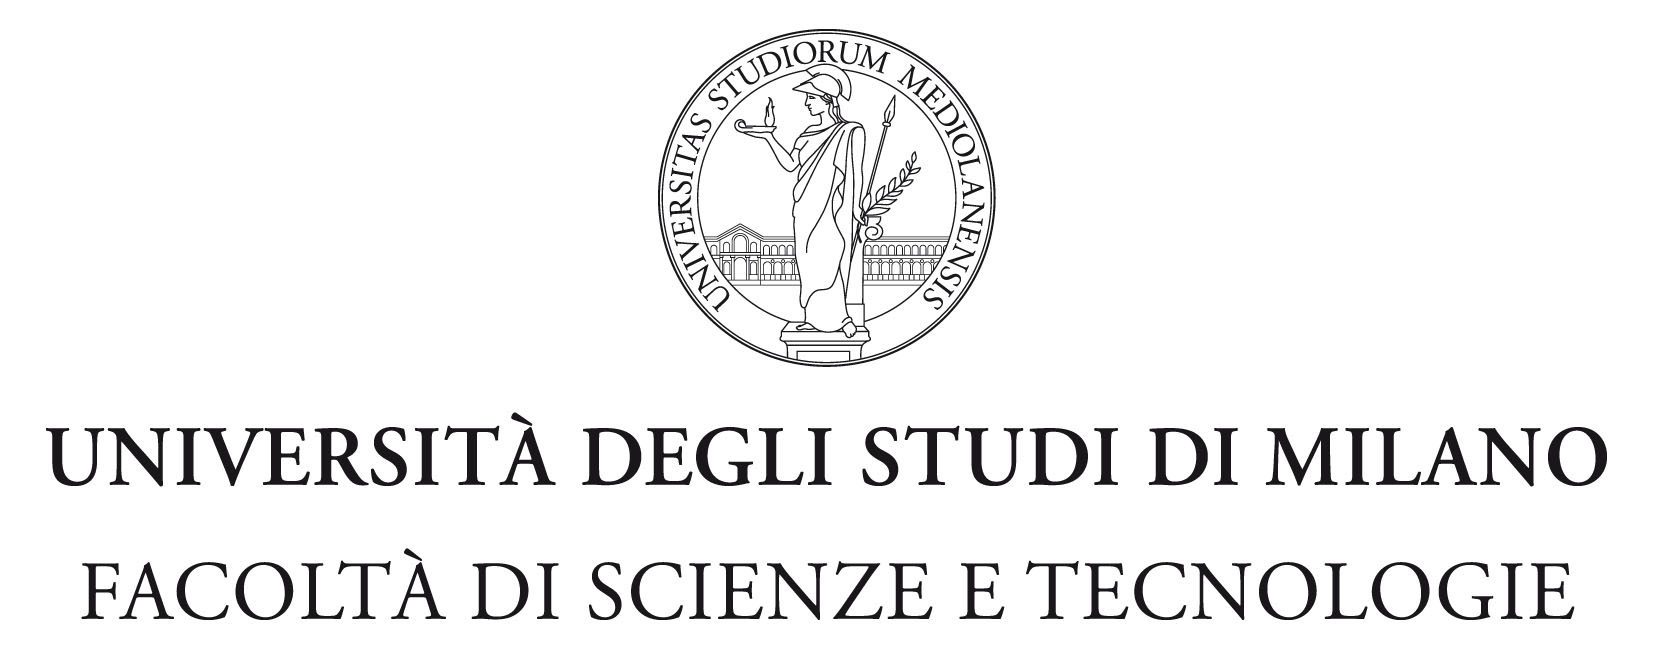
\includegraphics[width=390pt]{graphics/cover-page/logo.jpg}
		\centering
	%	\vspace{0.1 cm}
	\end{figure}	
\begin{center}
{\large Corso di Laurea Magistrale in Fisica}
\end{center}

\begin{center}
\vspace{2 cm}
{\Large \textsc{A study for the measurement of the $\Lambda$ baryon electromagnetic
dipole moments in LHC}b\par}
\end{center}
%\par
  \vspace{2 cm}
  
  \begin{flushleft}
  		 Relatore: \hskip 0.62 cm Prof. Nicola NERI\\
		 
  		 \noindent Correlatore: \hskip 0.1 cm Dott.ssa\ Elisabetta SPADARO NORELLA
  \end{flushleft}
  \vspace{1 cm}
  \begin{flushright}
  	Tesi di Laurea di:\\ Alessandro DE GENNARO\\ Matricola \hskip 0.1 cm 933289\\ Codice P.A.C.S.: \hskip 0.1 cm 14.20.-c
  \end{flushright}
    	  
%\vfill
\begin{center}
\vspace{2 cm}
{\large Anno Accademico 2020--2021}
\end{center}
\end{titlepage}